\newpage
\fancyhead[C]{Thomas Turner}
\section{Return to Safety} \label{Return to Safety}


\subsection{Introduction and Philosophy}
Traditionally \gls{RTH} is executed in commercial drone products in case of detected faults and errors. This is usually sufficient and convenient for the user. However, this specific use case provides cause to expand this functionality. In cases of partial thrust failure, provided it is not above the critical value needed to maintain stability, the \gls{UAV} will have to use less aggressive control in order to cause no further degeneration and compensate for lower actuator saturation levels. This makes the \gls{UAV} less robust to disturbances and therefore introduces a significant probability of crashing. Similarly, if the battery state of charge is depleting faster than predicted and hence causing a state of charge failure you can model this as a probability of failure at any given point given the unpredictability of degenerating cells \cite{cell stuff}. Lastly, if adverse weather conditions are detected causing instability, similarly to if there is partial thrust failure, the device can no longer be assumed to be robust to the environmental disturbances and has a significant probability of crashing. Given the difficulty of retrieval, this means that traditional \gls{RTH} is not the optimal strategy in these specific cases and instead a \gls{RTS} strategy is more appropriate.

\paragraph{When to use \gls{RTH}}
\gls{RTH} is always preferable to to \gls{RTS} as if you trace back the path you came down and return to the start location you can ensure that the path is obstacle free and you have returned to a safe and convenient location. Therefore, \gls{RTH} should be used when the probability of failure at any specific instant on the path is negligible as the drone is robust to the environmental conditions, and when the drone has accurate location sensing for avoidance of large obstacles and obstructions. This means in cases of redundant sensor or communication faults, non safety critical sensor faults, or if commanded by the base station, \gls{RTH} should be executed.

\paragraph{Objectives}
The objective of the \gls{RTS} system is to provide a robust and flexible procedure that can be operated from the flight controller with minimal added memory and time complexity that provides optimal or near optimal routes to safe landing zones. It should also be easy to setup and operate by untrained ground operators.


\subsection{Cost Maps}
\subsubsection{Source data}
When considering \gls{RTS} it requires prior knowledge of the operating environment which is loaded into the drone using ground operators before flight. This is accomplished using bird's eye images of the operating areas and marking the obstructions, suspected mined regions, mildly dangerous regions, and safe landing regions, with corresponding \gls{GNSS} co-ordinates.
\paragraph{Satellite Images}
Where satellite images are available and accurate they are the easiest option. However, given the nature of environments effected by war, there may have been significant changes to the local environment since the last satellite image. Furthermore, seasonal changes can make satellite images less effective as trees may be less visible from winter images due to a lack of leaves.
\paragraph{Surveillance Images}
Standard consumer level drones can provide images with tagged \gls{GNSS} co-ordinates that can be used, however, this requires extra hardware and time to execute. Therefore, this should be avoided where satellite images are sufficient.

\subsubsection{Graphical User Interface}
\paragraph{Platform} 
The \gls{GUI} was considered from the start to maximise usability by untrained ground operators. I built the \gls{GUI} using a simple python script that takes an image path and uses hardware-independent click locations and keystrokes to operate. It then gives the output as a $.txt$ file with a standard format. This means that the process can be run on any local hardware available.
\paragraph{User interactions}
The user can click on a region to set it a colour representing the classification, there is also a separate mode that uses intensities not colours to support colour-blind ground operators. Semi-transparent shades are used so the base image can be seen through the shade of classification colour allows for a more natural filling experience. Furthermore, some utility functions including multi-zone filling, clicking on already classified regions to deselect and auto-filling regions were added to make the process easier and faster. The process from satellite image (from Google Earth), to cost map, to a flow map is shown in \ref{fig:cost map net}. The only information uploaded to the drone is \ref{fig:cost map flow} where the arrows denote where to go next and the circles denote where, if there, the device should land.

\subsubsection{Tessellated surfacing}
\paragraph{Hexagons} While squares and triangles are more widely used, they are worse than hexagons for this application as they are less intuitive. Travelling centre to centre on the diagonals of squares goes through a point of four intersection where the classification is undefined. Therefore if the user added two obstacles diagonally connected it is unknown if you could travel diagonally between them, this ambiguity creates issues that you do not face when using hexagons as while at the intersections the classifications are still undefined, when travelling centre to centre you never cross an intersection of more than two hexagons.
\paragraph{Mapping hexagons to \gls{GNSS}} \label{para:Mapping hexagons}
The two key methods of mapping from hexagons to Cartesians either uses two axial co-ordinates or using row and column values with an offset described in previous work\cite{MappingHexagons}. Once the converted into Cartesian form you multiply the values by the scaling factor to get offset from the origin. This is combined with the known location of the origin to generate the \gls{GNSS} tags for the centre of each hexagon.

\subsubsection{Efficient filling}
\paragraph{Auto-filling from Path Planning}
Having the ground user filling in both the path planning polygonal zones and the cost map is inefficient due to the shared information. Therefore, provided the images used are the same, the cost map automatically classifies hexagons with an obstacle listed within its bounds as an obstacle region. It also automatically classifies the region of interest as dangerous to land as it is a mined area. This reduces the number of zones required to be filled by the ground operator. 
\paragraph{Dynamic Zooming}
In complicated operating environments higher resolutions may be needed, however, often the major zones will remain the same. Therefore, the user will have two different views, the major view that is used to fill in large zones and the minor view that the user accesses in order to fill in smaller more detailed zones. 
\paragraph{Machine Learning Methods}
The cost map generating program not only records the final results but all of the ground operator times and clicks. This output file is sent to the development team, if the ground user has not disabled this functionality due to safety or privacy reasons. This will support future work to create new tools to reduce the time taken in combination with feedback.
\begin{figure}[htbp]
  \centering
  \begin{subfigure}[b]{0.32\textwidth}
    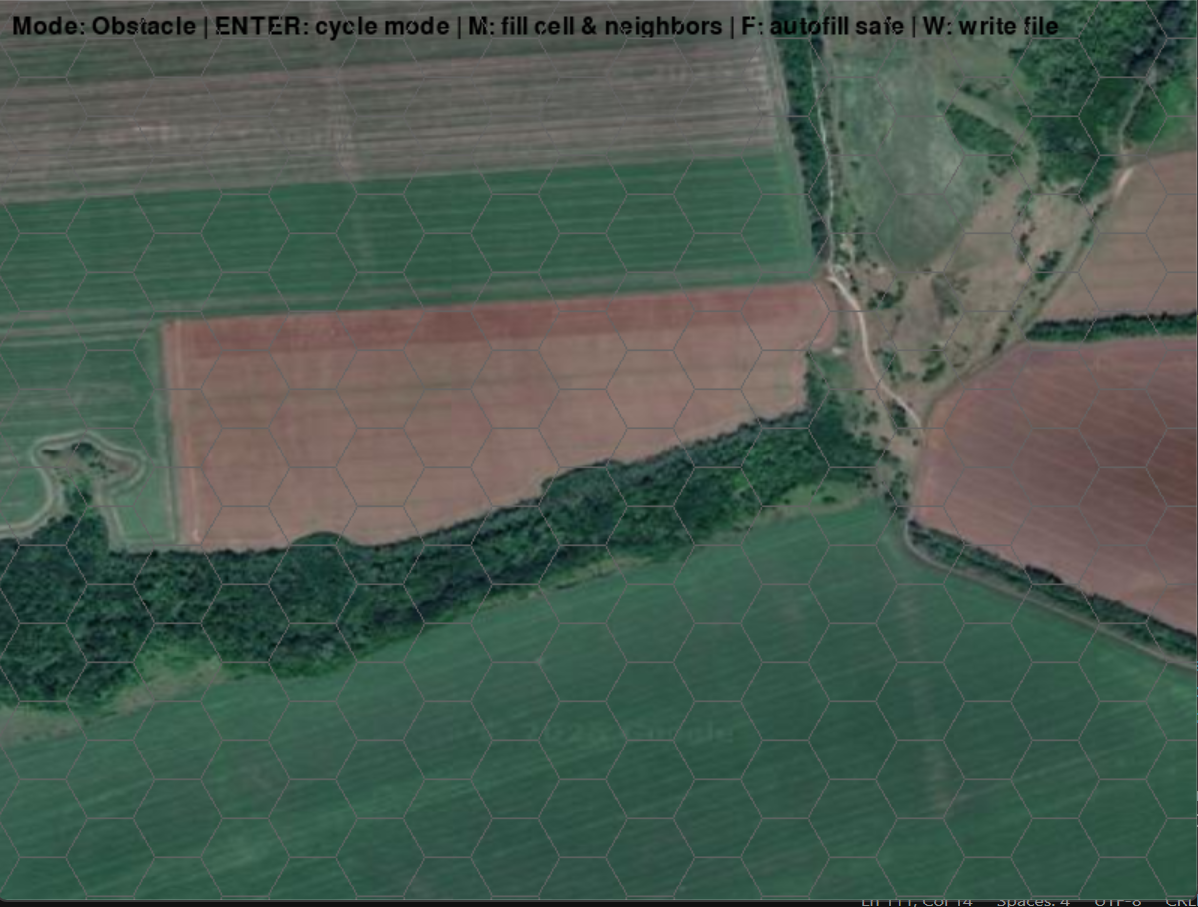
\includegraphics[width=\textwidth]{figs/Thomas/Return To Safety/50.19.27.N 36.55.32.E.png}
    \caption{Satellite Image}
    \label{fig:cost map satellite}
  \end{subfigure}
  \hfill
  \begin{subfigure}[b]{0.32\textwidth}
    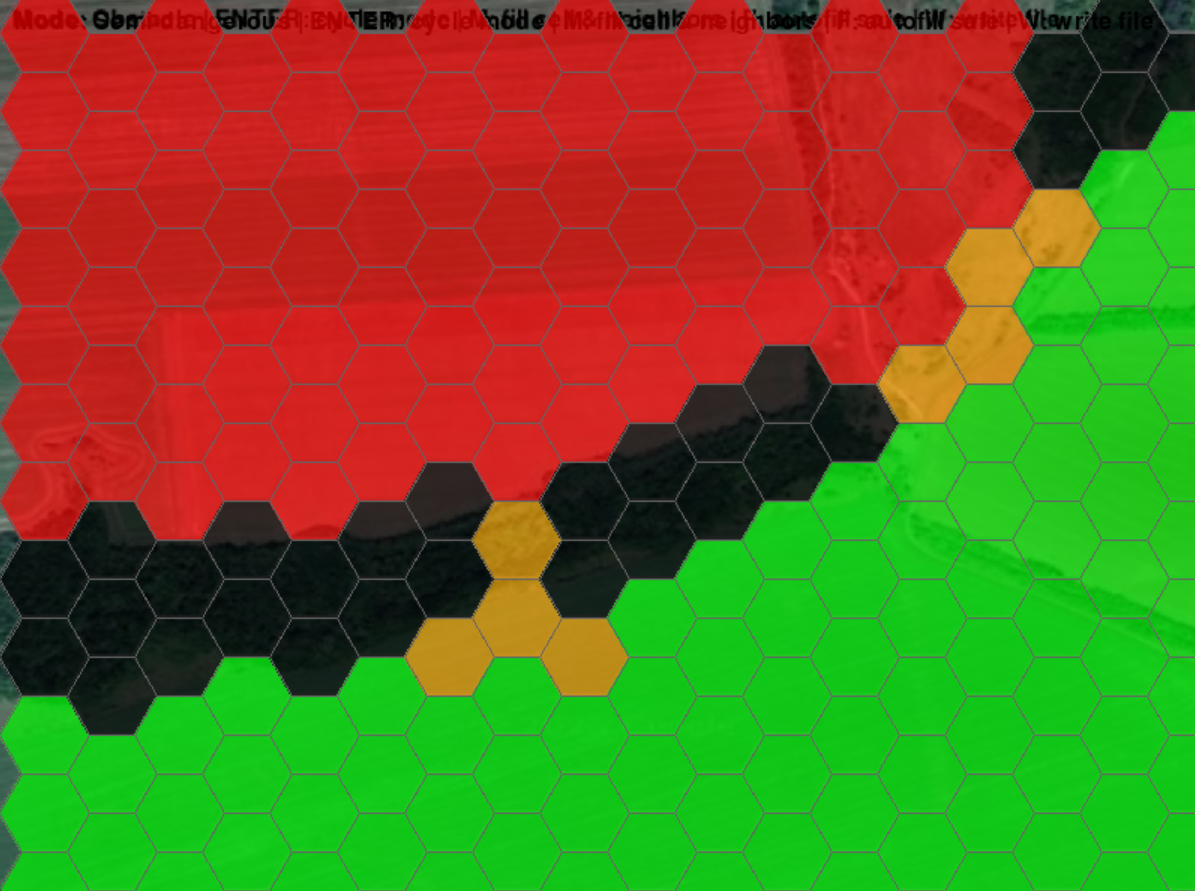
\includegraphics[width=\textwidth]{figs/Thomas/Return To Safety/50.19.27.N 36.55.32.E Cost.png}
    \caption{Cost Map}
    \label{fig:cost map cost}
  \end{subfigure}
  \hfill
  \begin{subfigure}[b]{0.32\textwidth}
    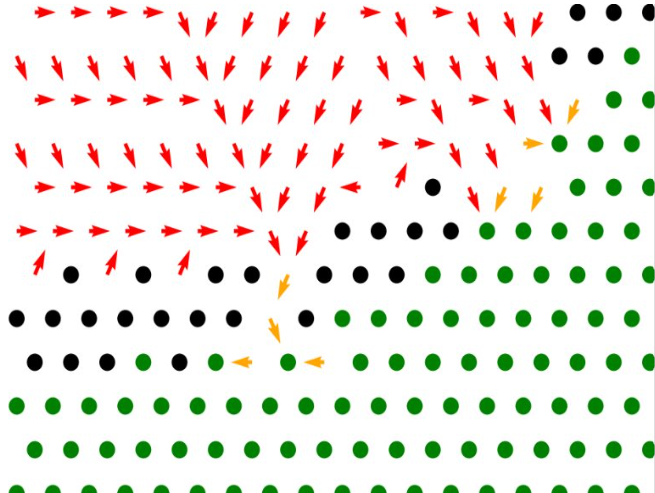
\includegraphics[width=\textwidth]{figs/Thomas/Return To Safety/50.19.27.N 36.55.32.E Flow.png}
    \caption{Flow Map}
    \label{fig:cost map flow}
  \end{subfigure}
  
  \caption{Geospatial analysis at coordinates 50.19.27.N 36.55.32.E}
  \label{fig:cost map net}
\end{figure}
\subsection{Emergency Path Planning}

\subsubsection{Objective and Cost Function}

\subsubsection{Search Algorithm}
\paragraph{Algorithm}
\paragraph{Complexity}

\subsubsection{Flow Algorithm}
\paragraph{Algorithm}
\paragraph{Complexity}

\subsection{Fault Detection, Quantification and Control}
\subsubsection{State of Charge}
\paragraph{Causes}
\paragraph{Modelling}

\subsubsection{Actuator Fault}
\paragraph{Causes}
\paragraph{Modelling}
\paragraph{Control Strategy}
\subsection{Simulation and Validation}
\subsubsection{Real-time application}
\subsubsection{Modelling Weather data}
 